\documentclass[twoside,twocolumn]{article}

\usepackage{blindtext} % Package to generate dummy text throughout this template 

\usepackage[sc]{mathpazo} % Use the Palatino font
\usepackage[T1]{fontenc} % Use 8-bit encoding that has 256 glyphs
\linespread{1.05} % Line spacing - Palatino needs more space between lines
\usepackage{microtype} % Slightly tweak font spacing for aesthetics

\usepackage[english]{babel} % Language hyphenation and typographical rules

\usepackage{graphicx}
\usepackage{booktabs}
\usepackage{amsmath, amsthm, amssymb, bm}
\usepackage{tikz, pgfplots}
\usepackage{float}

\usepackage[hmarginratio=1:1,top=32mm,columnsep=20pt]{geometry} % Document margins
\usepackage[hang, small,labelfont=bf,up,textfont=it,up]{caption} % Custom captions under/above floats in tables or figures
\usepackage{booktabs} % Horizontal rules in tables

\usepackage{lettrine} % The lettrine is the first enlarged letter at the beginning of the text

\usepackage{enumitem} % Customized lists
\setlist[itemize]{noitemsep} % Make itemize lists more compact

\usepackage{abstract} % Allows abstract customization
\renewcommand{\abstractnamefont}{\normalfont\bfseries} % Set the "Abstract" text to bold
\renewcommand{\abstracttextfont}{\normalfont\small\itshape} % Set the abstract itself to small italic text

\usepackage{titlesec} % Allows customization of titles
\renewcommand\thesection{\Roman{section}} % Roman numerals for the sections
\renewcommand\thesubsection{\roman{subsection}} % roman numerals for subsections
\titleformat{\section}[block]{\large\scshape\centering}{\thesection.}{1em}{} % Change the look of the section titles
\titleformat{\subsection}[block]{\large}{\thesubsection.}{1em}{} % Change the look of the section titles

\usepackage{fancyhdr} % Headers and footers
\pagestyle{fancy} % All pages have headers and footers
\fancyhead{} % Blank out the default header
\fancyfoot{} % Blank out the default footer
\fancyhead[C]{Running title $\bullet$ May 2016 $\bullet$ Vol. XXI, No. 1} % Custom header text
\fancyfoot[RO,LE]{\thepage} % Custom footer text

\usepackage{titling} % Customizing the title section

\usepackage{hyperref} % For hyperlinks in the PDF

\newtheorem{theorem}{Theorem}[section]
\newtheorem{corollary}{Corollary}[theorem]
\newtheorem{lemma}[theorem]{Lemma}
\renewcommand{\vec}[1]{\underline{#1}}
\newcommand\twospace{\,\,}
\newcommand\fourspace{\,\,\,\,}
\newcommand\norm[1]{\ensuremath{\lVert#1\rVert_2}}
\newcommand\abs[1]{\ensuremath{\Vert#1\Vert}}
%----------------------------------------------------------------------------------------
%	TITLE SECTION
%----------------------------------------------------------------------------------------

\setlength{\droptitle}{-4\baselineskip} % Move the title up

\pretitle{\begin{center}\Huge\bfseries} % Article title formatting
\posttitle{\end{center}} % Article title closing formatting
\title{Subgradient Method} % Article title
\author{%
\normalsize Indian Institute of Technology, Hyderabad \\ % Your institution
\normalsize \href{mailto:ai20btech11006@iith.ac.in}{ai20btech11006@iith.ac.in} % Your email address
%\and % Uncomment if 2 authors are required, duplicate these 4 lines if more
%\textsc{Jane Smith}\thanks{Corresponding author} \\[1ex] % Second author's name
%\normalsize University of Utah \\ % Second author's institution
%\normalsize \href{mailto:jane@smith.com}{jane@smith.com} % Second author's email address
}
\date{\today} % Leave empty to omit a date
\renewcommand{\maketitlehookd}{%
\begin{abstract}
\noindent
Non-differentiable functions are an important class of functions which often appear in optimization problems, a gradient descent method would fail to optimize such an objective because the gradient might not exist at all points that the method encounters. Methods such as interior point method work great, but it has its own limitations of being computationally inefficient. We will explore the subgradient method which is an iterative first-order method similar to gradient descent. 
\end{abstract}
}

%----------------------------------------------------------------------------------------

\begin{document}

% Print the title
\maketitle

\section{Introduction}
Subgradient method is a simple algorithm used to minimize non-differentiable convex functions. This method is similar to vanilla gradient method which is used to optimize differentiable functions. 
% can add few lines on comparison

\subsection{Algorithm}
Lets say we have a nondifferentiable function $f\, : \, \mathbb{R}^n\to \mathbb{R}$. The update rule of subgradient method says
\begin{align}
    \vec{x}^{(k+1)} = \vec{x}^{(k)} - \alpha_k\vec{g}^{(k)} \label{eq:subgrad_iter}
\end{align}
where $\vec{x}^{(k)}$ is the $k^{th}$ iterate, $\alpha_k$ is the step step size at $k^{th}$ iteration and $\vec{g}^{(k)}$ is any subgradient of $f$ at $\vec{x}^{(k)}$. The subgradient $\vec{g}^{(k)}$ is any vector which satisfies
\begin{align}
    f(\vec{y}) \geq f(\vec{x}) + \vec{g}^T(\vec{y}-\vec{x})\label{eq:subgrad_condition}
\end{align}
At a given pozint there can be more than one subgradients, we call the set of subgradients as subdifferential.
\begin{theorem}
    If the function f is differentiable at $\vec{x}^{(k)}$ then $\vec{g}^{(k)}$ is equal to the gradient of f at $\vec{x}^{(k)}$
\end{theorem}
\begin{proof}
    Substitute $\vec{y} = \vec{x}+\lambda\vec{z},\twospace \lambda > 0$ in \eqref{eq:subgrad_condition}
    \begin{align}
        \frac{f(\vec{x}+\lambda\vec{z}) - f(\vec{x})}{\lambda} \geq \vec{g}^T\vec{z}
    \end{align}
    We can use the limit $\lambda \to 0$
    \begin{align}
        \vec{\nabla}f(\vec{x})^T\vec{z} &\geq \vec{g}^T\vec{z}\\
        \vec{z}^T\left(\vec{\nabla}f(\vec{x})-\vec{g}\right) &\geq 0 \fourspace \forall \vec{z}\\
        \therefore \vec{g} & = \vec{\nabla}f(\vec{x})
    \end{align}
\end{proof}

\section{Example}
Consider the following problem

\begin{align}
    min\fourspace max\{f_1,f_2,\dots f_n\}
\end{align}
This problem is non differentiable but it can be solved using subgradient method. Lets consider a numerical example.

\section{Convergence proof}
Lets assume $x^*$ is the minimizer of our objective function $f$. Assume that the norm of subgradients is bounded.

Using Lipschitz condition
\begin{align}
    \left| f(u)-f(v)\right| \leq G\norm{u-v}
\end{align}
for all $u,v$. Some versions of subgradient method work even when the gradient is not bounded. 

\section{SVM using subgradient method}
A support vector machine is used for two class classification. The objective is to maximize the slab thickness while still satisfying  few constraints. A hard-margin SVM can be formuated as
\begin{align}
    \begin{split}
        \min_{\vec{w},b}\, &\twospace\vec{w}^T\vec{w}
    \end{split}\\ 
    \text{s.t:}
    \twospace & y_i(\vec{w}^T\vec{x_i}+b)\geq 1\\
\end{align}
We can transform this problem into
\begin{align}
    \min_{\vec{w},b}\, &\twospace\vec{w}^T\vec{w} + \lambda \sum_i \max(0, 1-y_i\left(\vec{w}^T\vec{x}+b\right)
\end{align}
Where $\lambda$ is the trade off factor, the higher is the value of this parameter, the higher is the penalty of voilating the given constraints. This problem is essentially a soft-margin SVM. We can now solve this problem by subgradient method.

The first step is to calculate the subgradients, 
\begin{align}
    \vec{g}_{\vec{w}} = 2*\vec{w}+\lambda\displaystyle\sum_i y_i*\vec{x_i} \fourspace for\,  y_i\left(\vec{w}^T\vec{x}+b\right) < 1
\end{align}
and
\begin{align}
    g_{b} = \lambda\displaystyle\sum_i y_i \fourspace for\,  y_i\left(\vec{w}^T\vec{x}+b\right) < 1
\end{align}
In practice, we tend to use mini-batch subgradient method because of its several advantages such as computational efficiency, stable convergence and faster learning.

\section{Results}
\subsection{Maximum of convex functions}
I considered a problem of the type maximum of linear functions and compared different step size rules. The results obtained are as follows
\begin{enumerate}
    \item Constant Step Size
    \begin{figure}[H]
        \centering
        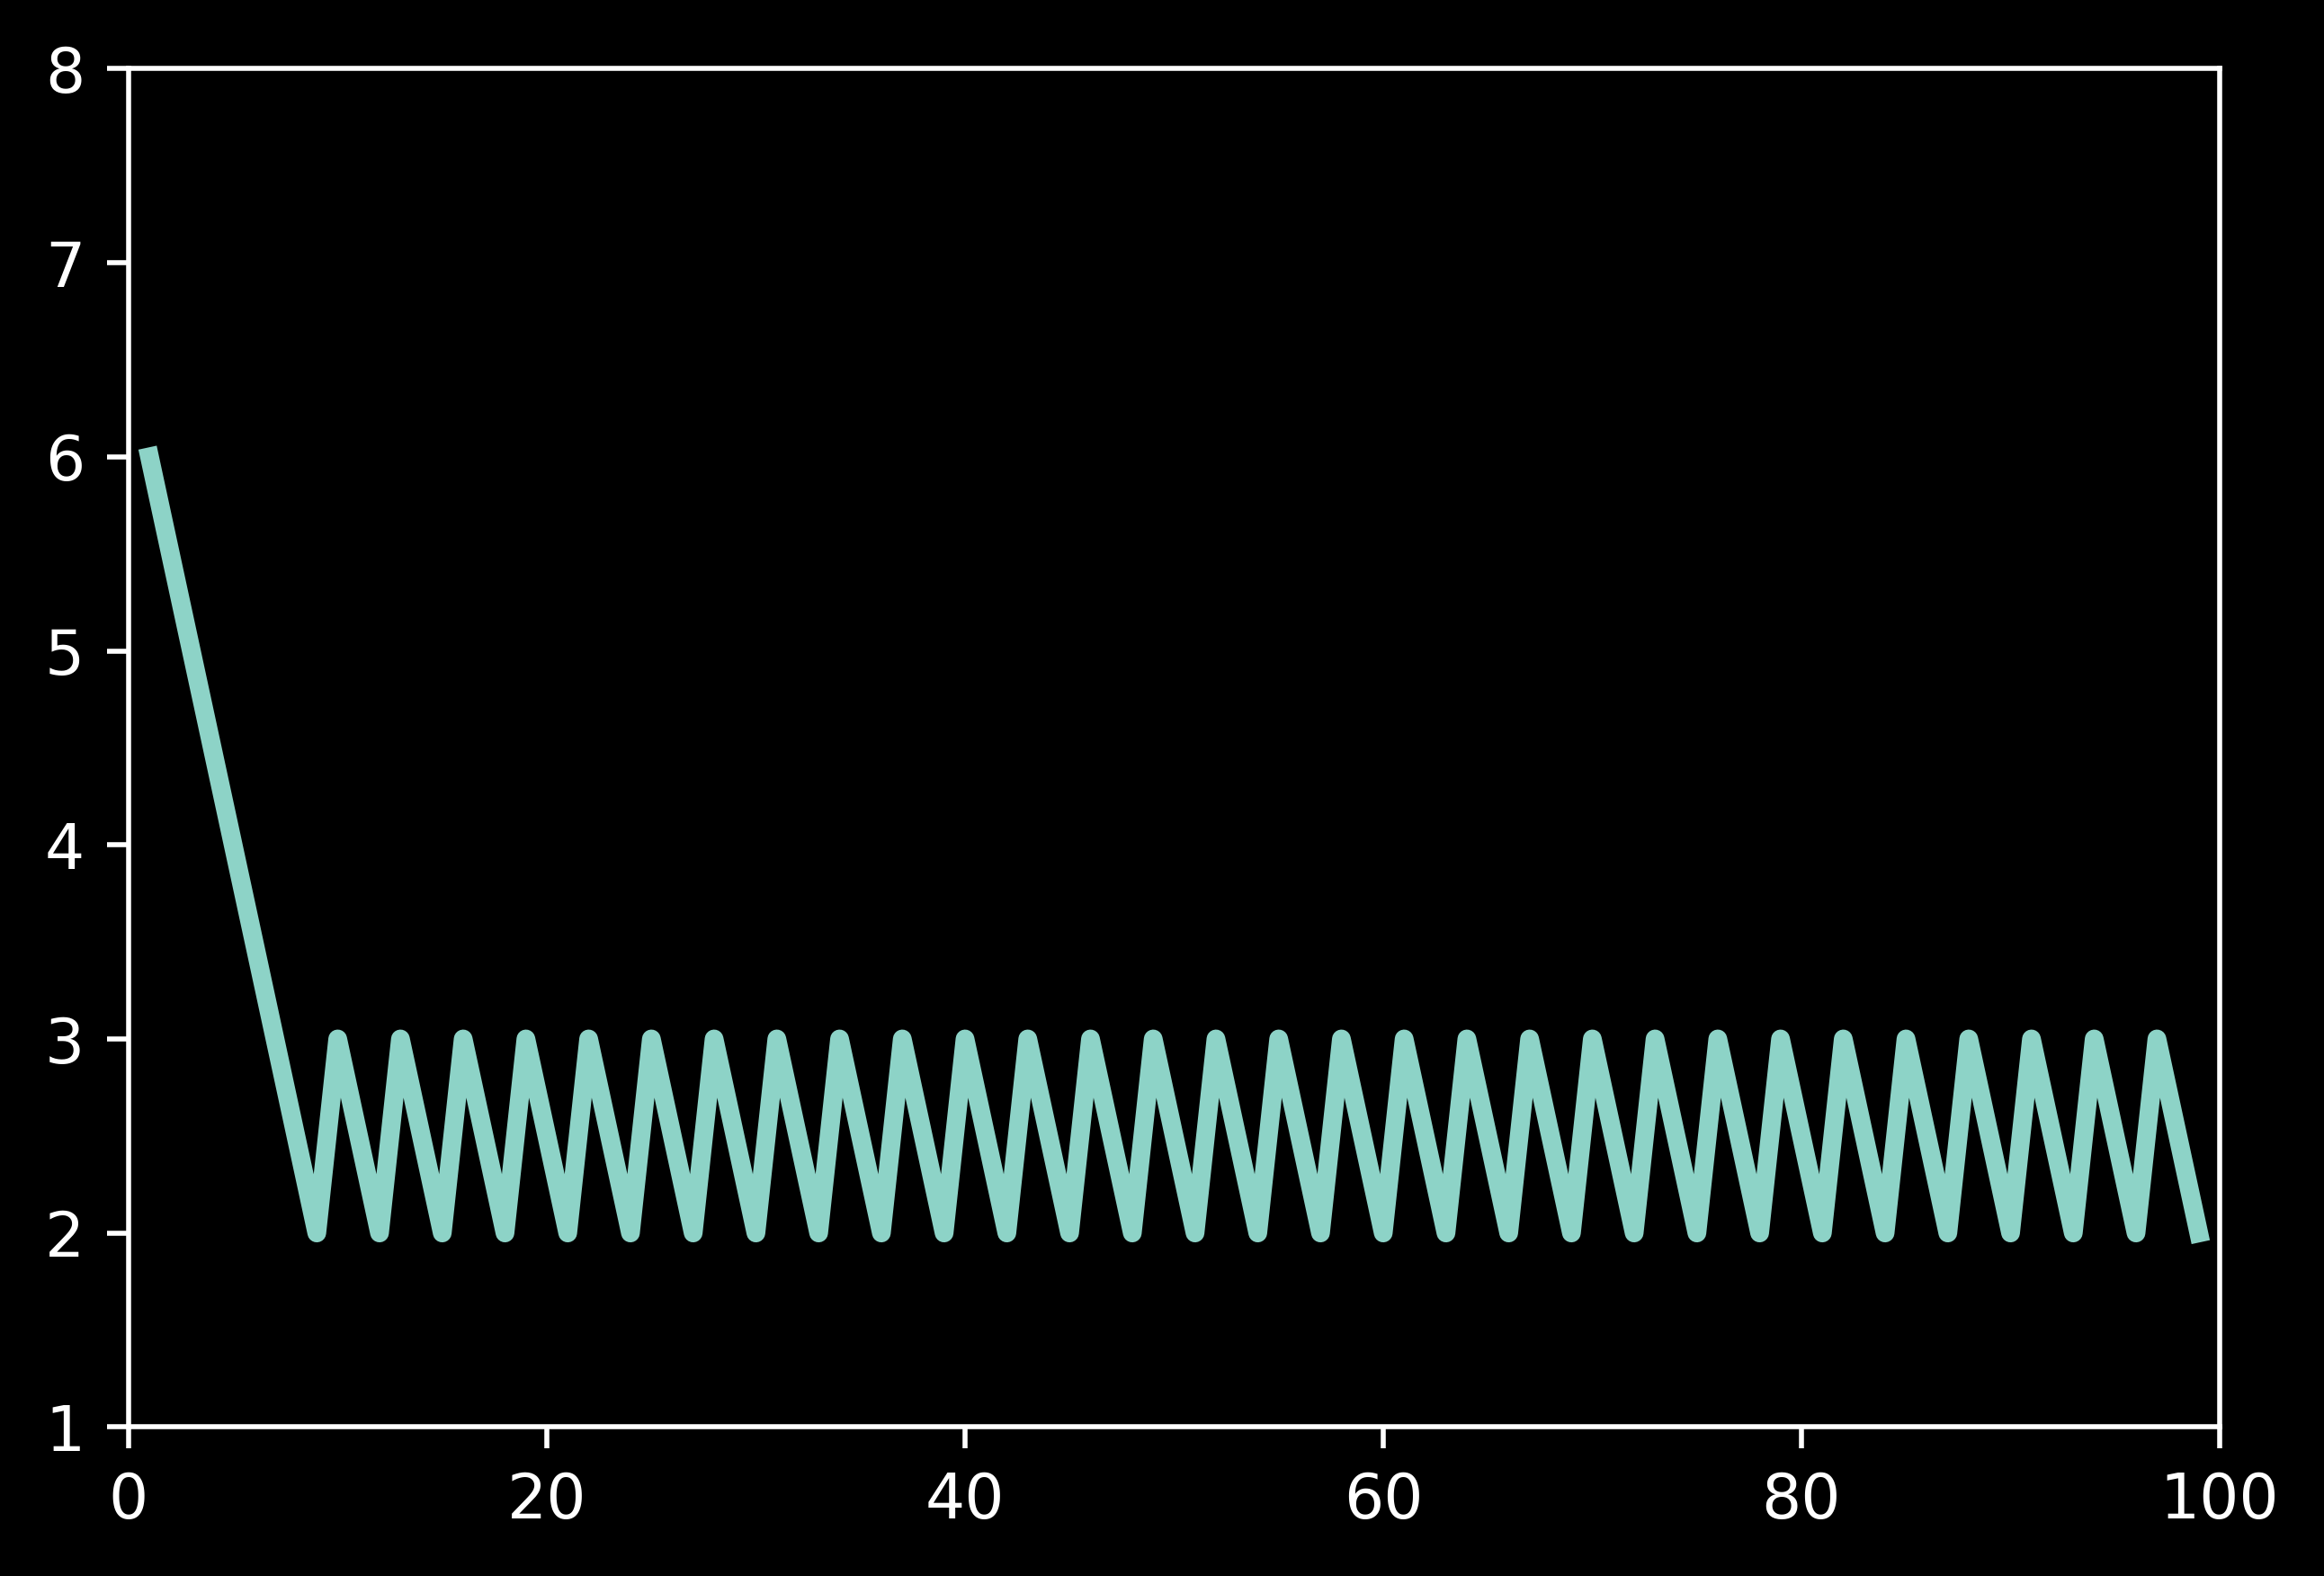
\includegraphics[scale=0.5]{../../step/constantstepsize.png}
        \caption{Constant Step Size}
        \label{constantstepsize}
    \end{figure}
    \item Constant Step Length
    \begin{figure}[H]
        \centering
        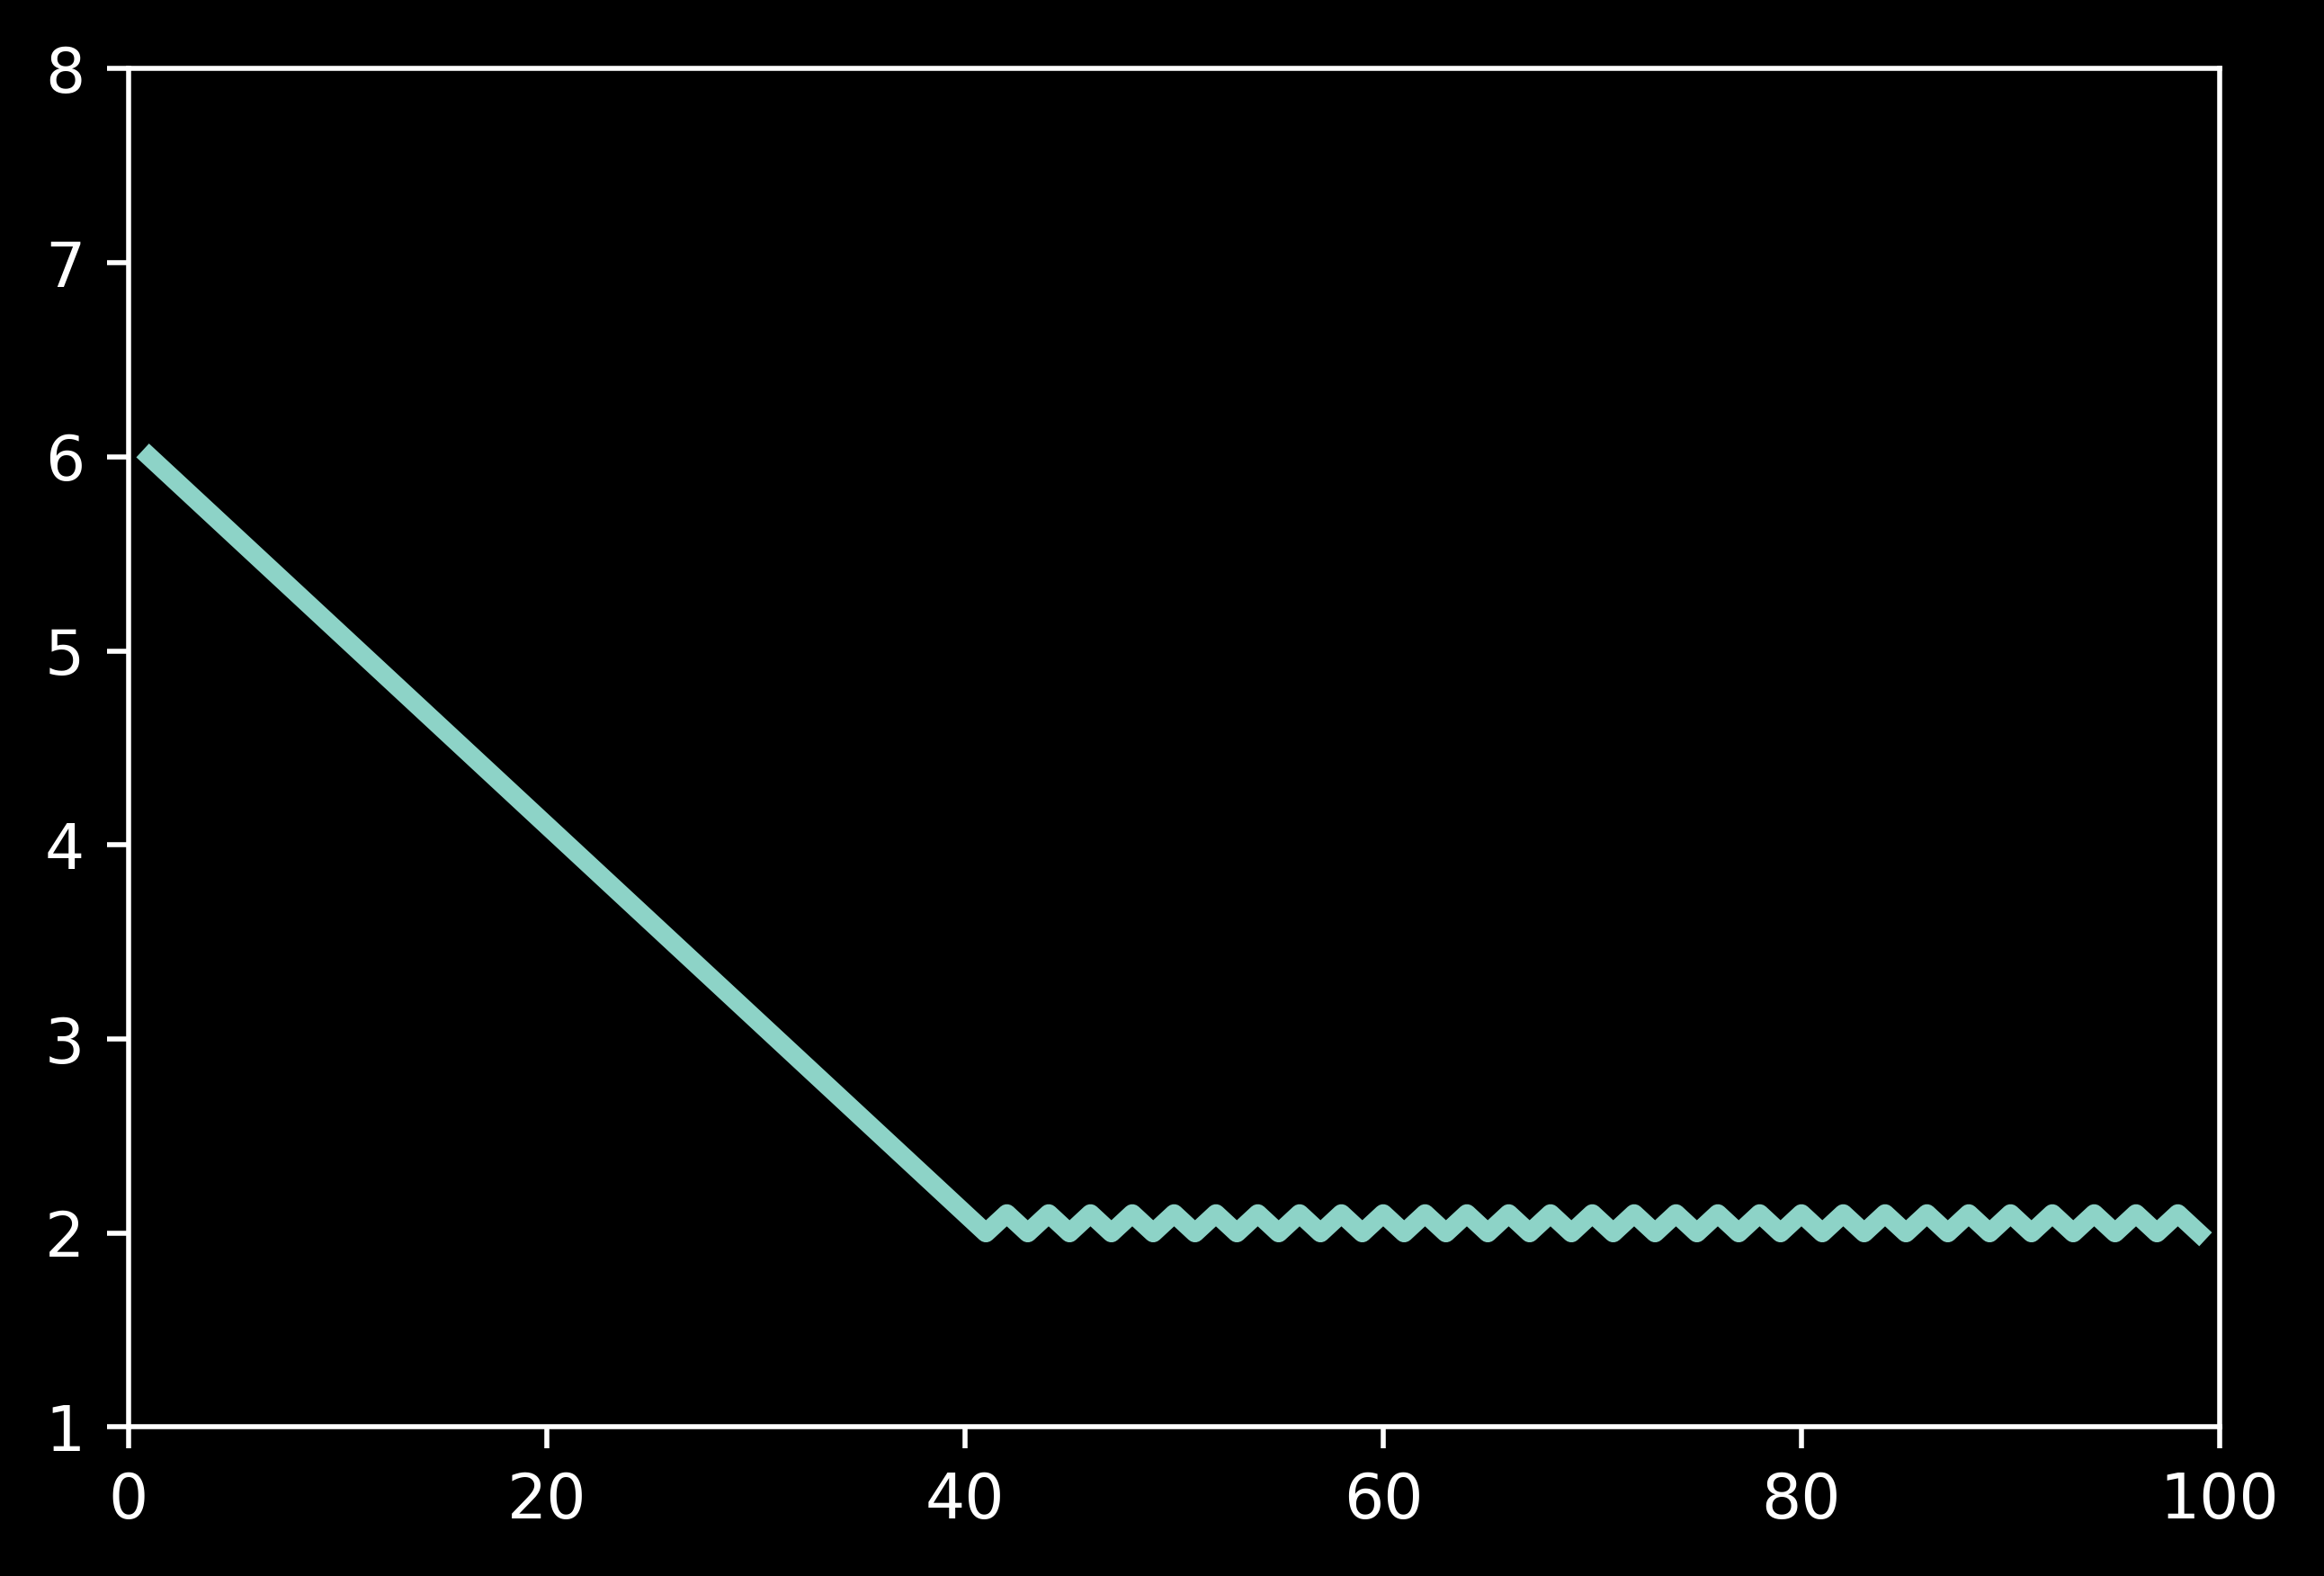
\includegraphics[scale=0.5]{../../step/constantsteplength.png}
        \caption{Constant Step Length}
        \label{constantsteplength}
    \end{figure}
    \item Square Summable But Not Summable
    \begin{figure}[H]
        \centering
        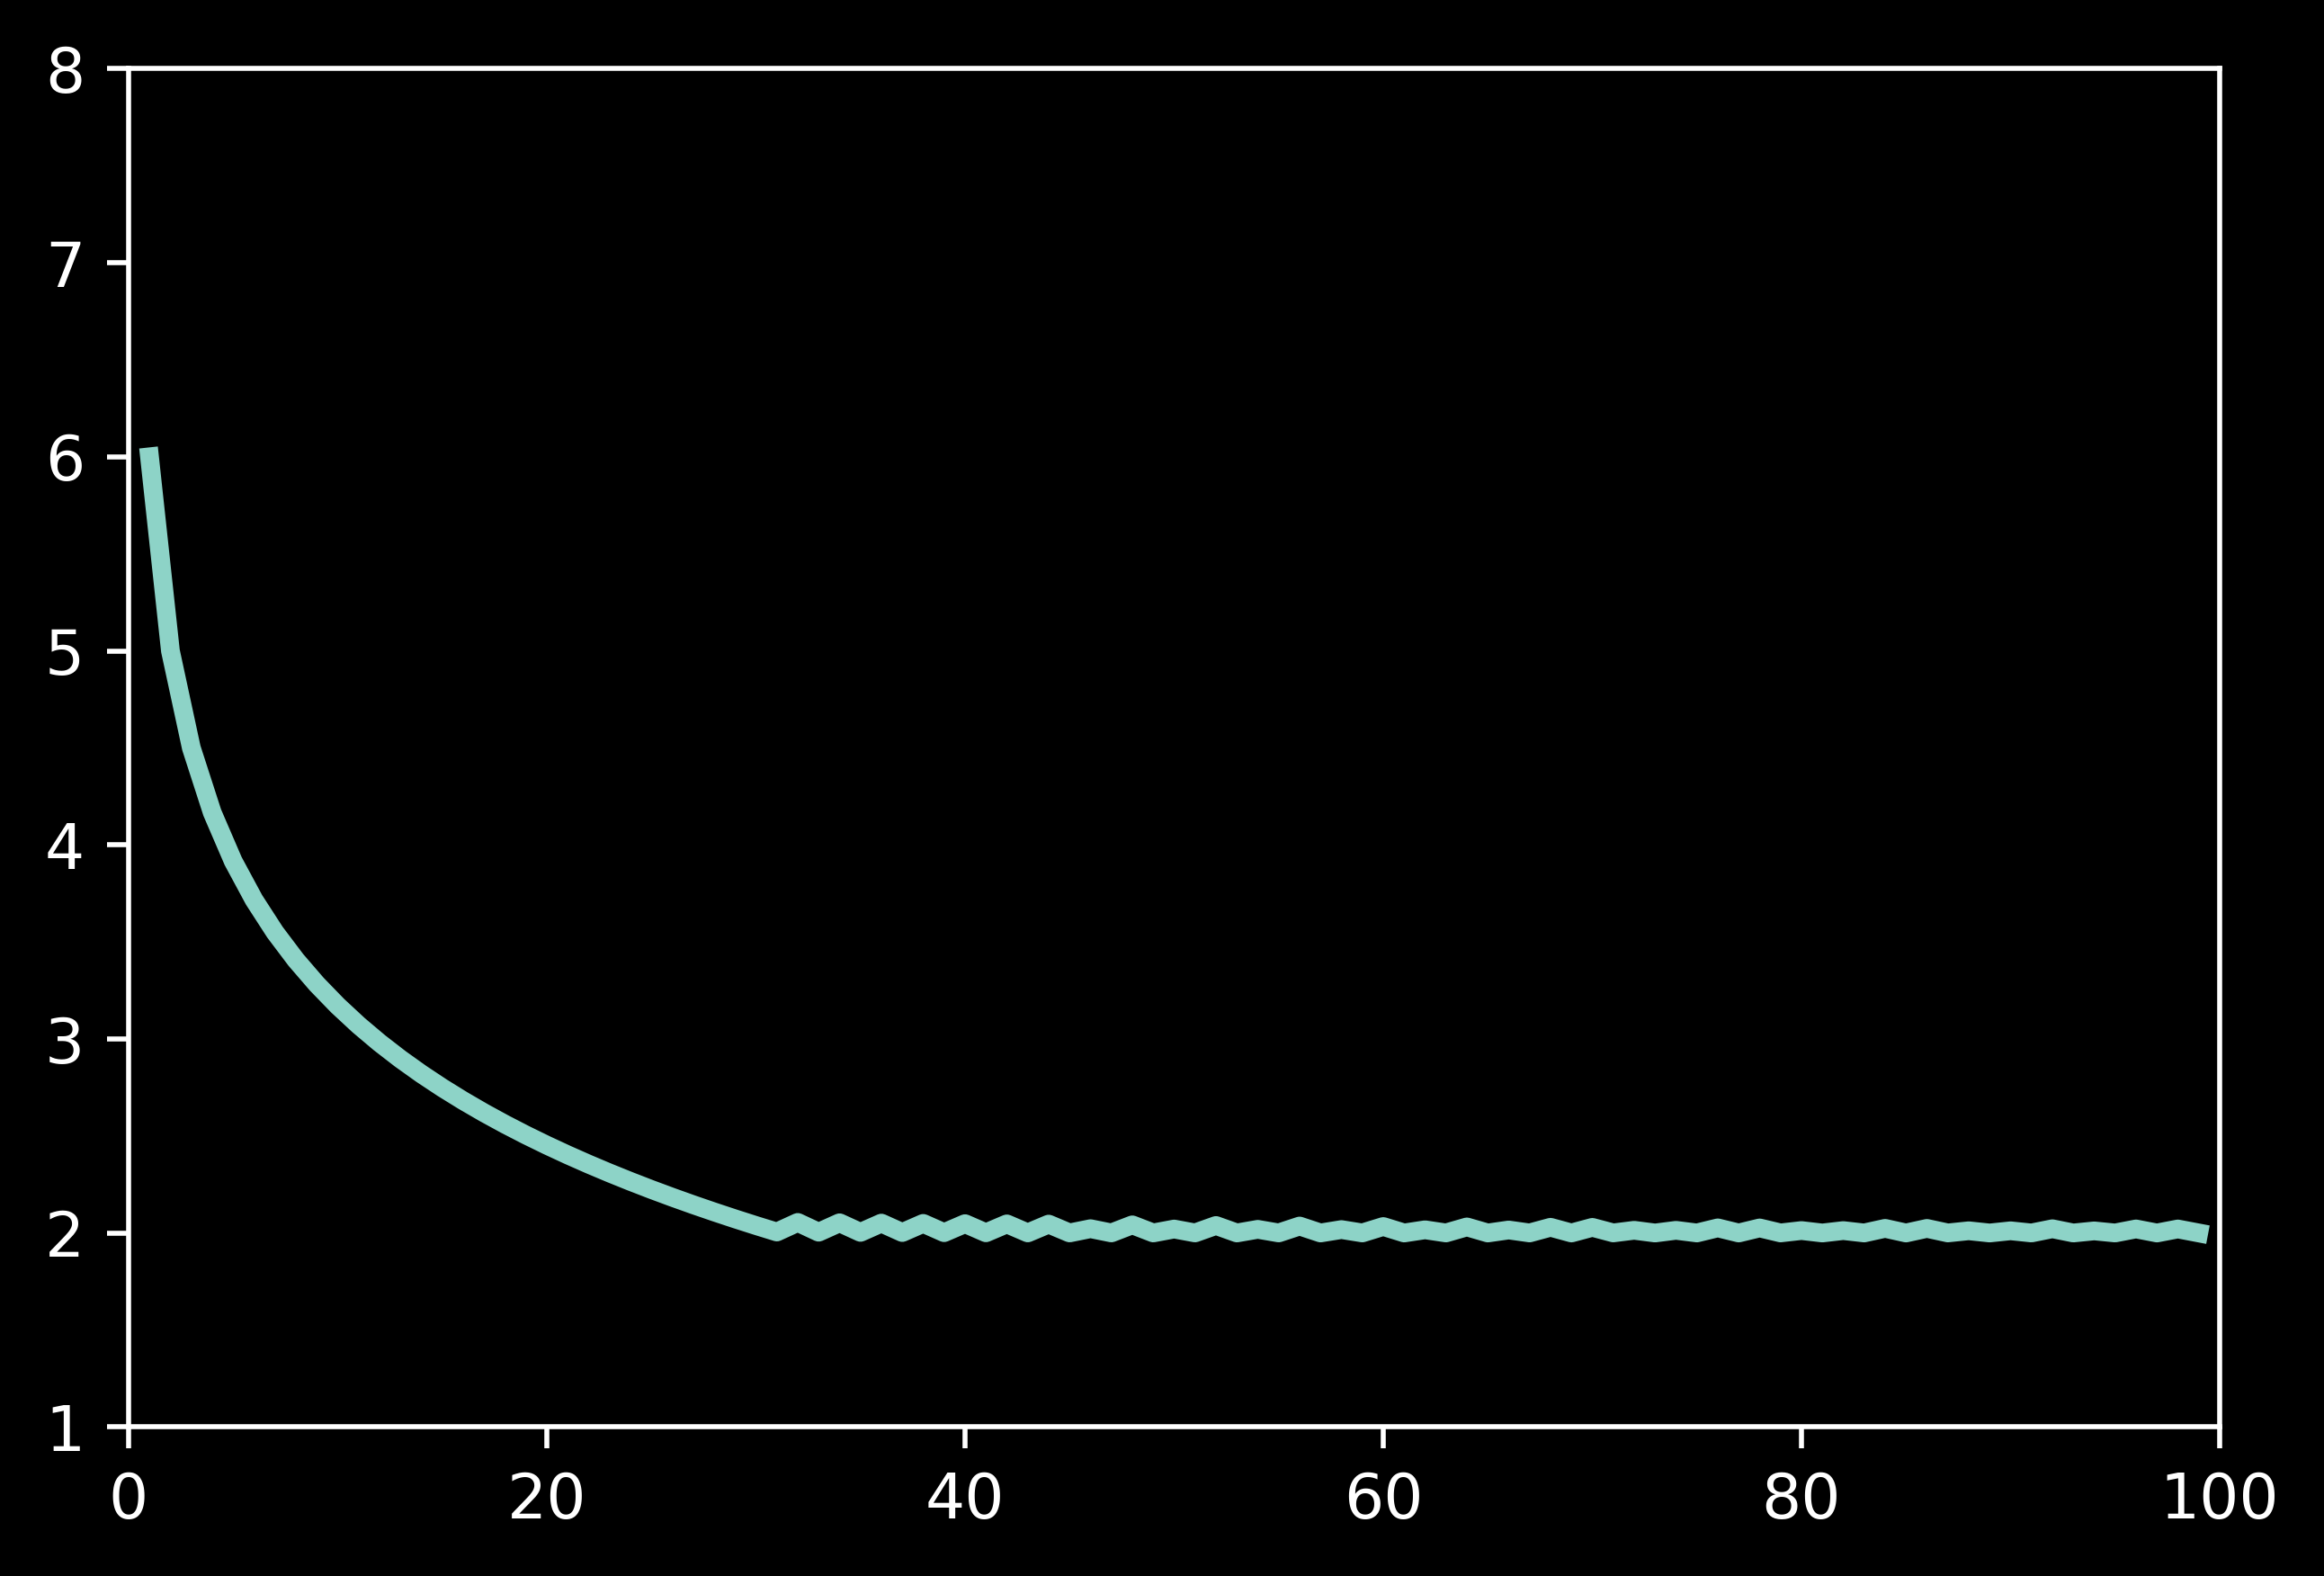
\includegraphics[scale=0.5]{../../step/squaresummablebutnotsummable.png}
        \caption{Square Summable But Not Summable}
        \label{squaresummablebutnotsummable}
    \end{figure}
    \item Non Summable Diminishing
    \begin{figure}[H]
        \centering
        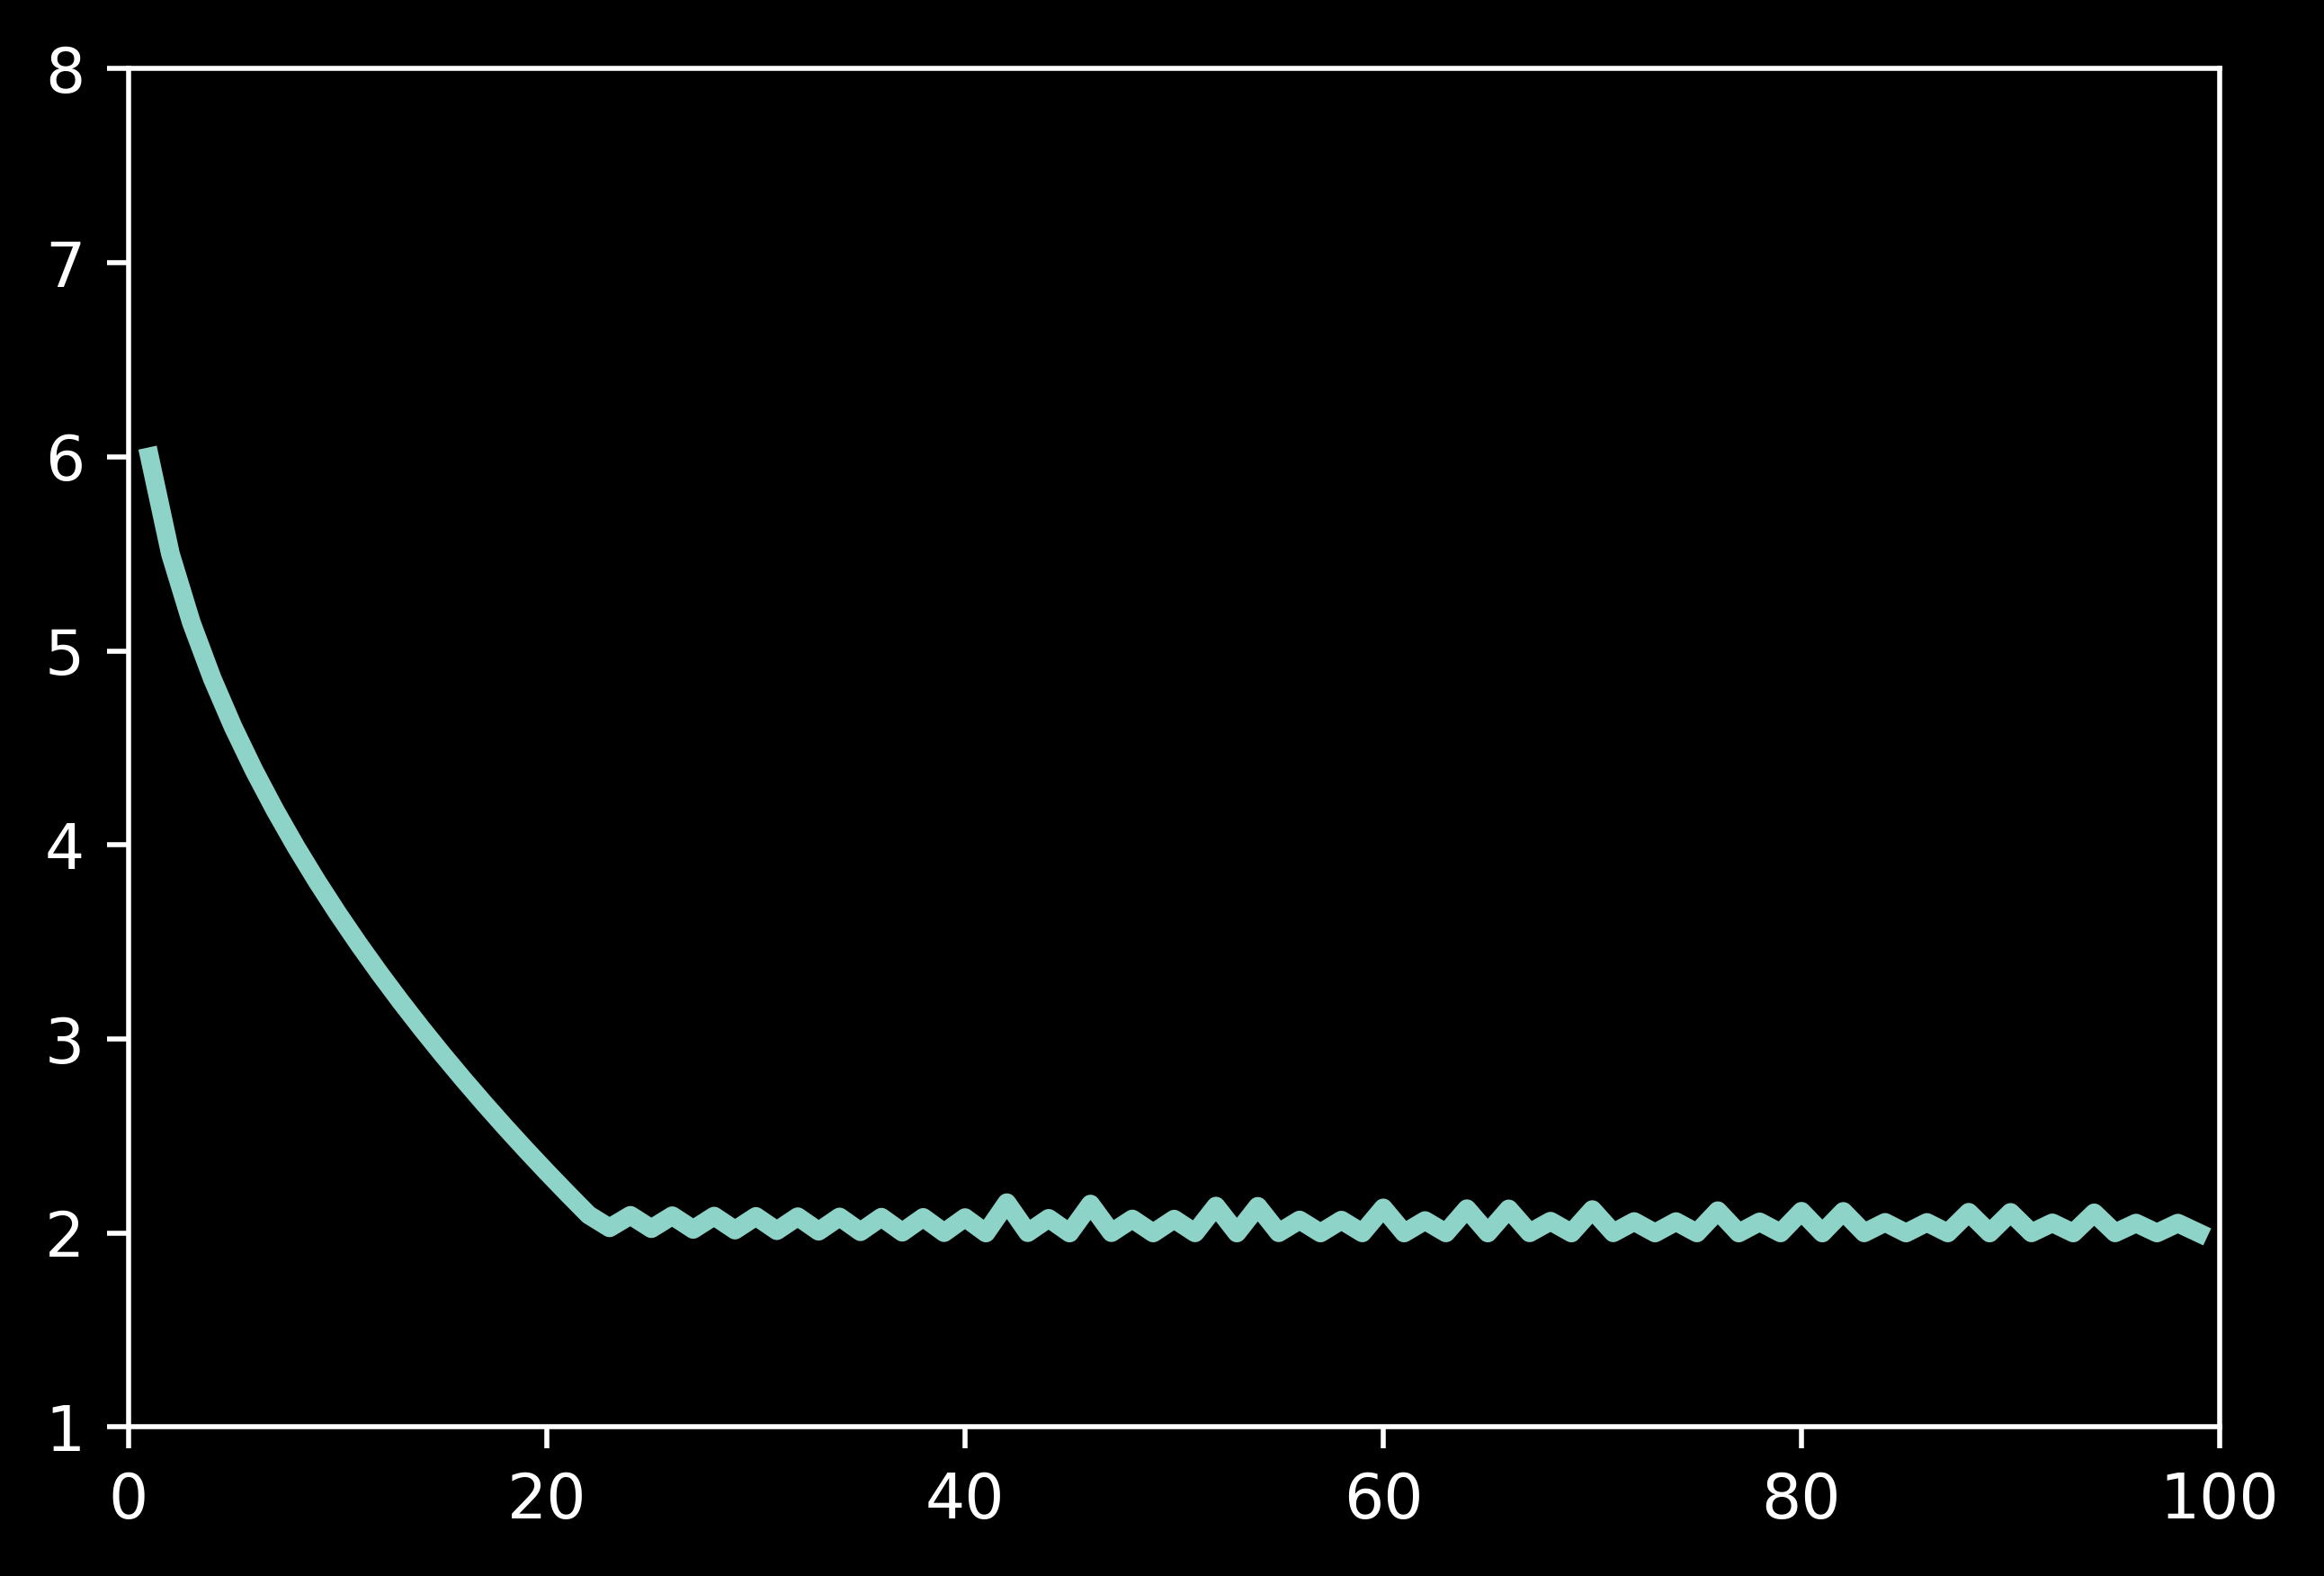
\includegraphics[scale=0.5]{../../step/nonsummablediminishing.png}
        \caption{Non summable diminishing}
        \label{nonsummablediminishing}
    \end{figure}
\end{enumerate}
We can see the difference in convergence across different step size rules.

The link to original code can be found \href{https://github.com/cmaspi/subgradient_method/blob/main/code/step_illustration.ipynb}{here} and the mp4 animation files can be found \href{https://github.com/cmaspi/subgradient_method/tree/main/results}{here}.

\subsection{SVM}
\subsubsection{Spam Classification}
Spam classification problem can be solved by soft margin SVM using linear kernel. The text in email can be tokenized and encoded in higher dimension. For our purposes, \emph{sklearn.feature\_extraction.text.CountVectorizer}~\cite{scikit-learn} can be used  
    

    


% expected structure
%-----------

% motivation for subgradient method
% a simple example where gradient descent wouldn't work

% correctness proof

% comparison with newton's method and interior point method

% A demonstration of sub gradient descent

% Applying subgradient descent in SVM

% Trying subgradient descent with other standard methods in gradient descent
% such as momentum ( heavy ball method)



%----------------------------------------------------------------------------------------
%	ARTICLE CONTENTS
%----------------------------------------------------------------------------------------
%-----------------------------------------------------------------
%	REFERENCE LIST
%----------------------------------------------------------------------------------------
{\small
\bibliographystyle{ieee_fullname}
\bibliography{egbib}
}

\section{References}
\begin{enumerate}
    \item Boyd, Stephen and Xiao, Lin and Mutapcic, Almir. Subgradient method \href{https://info.usherbrooke.ca/jpdussault/ROP771H17/subgrad_method_notes.pdf}{$^1$}
    \item Boyd, Stephen and Mutapcic, Almir. stochastic Subgradient method \href{https://web.stanford.edu/class/ee364b/lectures/stoch_subgrad_notes.pdf}{$^2$}
    \item edregosa, F. and Varoquaux, G. and Gramfort, A. and Michel, V.
    and Thirion, B. and Grisel, O. and Blondel, M. and Prettenhofer, P.
    and Weiss, R. and Dubourg, V. and Vanderplas, J. and Passos, A. and
    Cournapeau, D. and Brucher, M. and Perrot, M. and Duchesnay, E. Scikit-learn: Machine Learning in \{P\}ython\} $^3$
\end{enumerate}


\end{document}
